\documentclass[tikz,border=2]{standalone}
%
%%%%%%%%%%%%%%%%%%%%%%%%%%%%%%%%%%%%
%% Common preamble
%%%%%%%%%%%%%%%%%%%%%%%%%%%%%%%%%%%%
% PAGE
%% \usepackage{fullpage}
% FONTS
\usepackage{lmodern} % enhanced version of computer modern
\usepackage[T1]{fontenc} % for hyphenated characters
%% \usepackage{gillius2}
%% \renewcommand{\familydefault}{\sfdefault}
\usepackage{amssymb}
\usepackage{mathtools} % contains amsmath which comes with align
\usepackage{amsthm}
%%\usepackage{enumitem}
\usepackage{microtype} % some compression
%%%%%%%%%%%%%%%%%%%%%%%%%%%%%%%%%%%%
\usepackage{subfig}
\usepackage{tikz}
\usetikzlibrary{spy,shadows,arrows,shapes,positioning,calc,backgrounds,fit,automata}
\newcommand{\score}{\text{score}}

\definecolor{myblue}{HTML}{C5E0DC}
\definecolor{vtblue}{HTML}{557082}
\definecolor{hokie}{HTML}{660000}
\definecolor{hokieRed}{HTML}{980000}

\definecolor{col1}{HTML}{D53E4F}
\definecolor{col2}{HTML}{F46D43}
\definecolor{col3}{HTML}{FDAE61}
\definecolor{col4}{HTML}{FEE08B}
\definecolor{col5}{HTML}{E6F598}
\definecolor{col6}{HTML}{ABDDA4}
\definecolor{col7}{HTML}{66C2A5}
\definecolor{col8}{HTML}{3288BD}

\newcommand{\dunder}[1]{\underline{\underline{#1}}}
\newcommand{\dmax}{d_{\max}}
\newcommand{\cost}{\text{cost}}
\newcommand{\comment}[1]{{\color{red}#1}}
\newcommand{\wmin}{w_{\min}}
\newcommand{\copt}{C_{\text{OPT}}}
\newcommand{\TikZ}{Ti\textit{k}Z\xspace}
\newcommand{\tuta}{\emph{T. absoluta}}
\newcommand{\prempt}{\textsc{PREMpT}}

%% ----------------------------------------------------------------------
%%
\begin{document}
%%
%% ----------------------------------------------------------------------
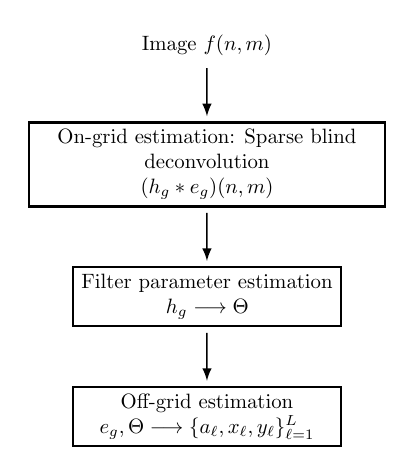
\begin{tikzpicture}
[scale=.75,auto,transform shape,
edge/.style={>=latex, shorten >=2pt, shorten <=2pt, line width=.2mm},
block/.style={draw=black,thick}]
\node (input) {Image $f(n,m)$};
\node (sbd) [block,minimum width=6cm,below=of input]{\parbox{5.8cm}{
\centering
On-grid estimation: Sparse blind deconvolution \\
$(h_g\ast e_g)(n,m)$
}};
%%
\draw[edge,->] (input) -- (sbd);
%%
\node (parEst) [block,minimum width=4.5cm,below=of sbd] {\parbox{4.3cm}{
\centering
Filter parameter estimation \\
$h_g\longrightarrow \Theta$
}};
%%
\draw[edge,->] (sbd) -- (parEst);
%%
\node (offGrid) [block,minimum width=4.5cm,below=of parEst]{\parbox{4.3cm}{
\centering
Off-grid estimation \\
$e_g,\Theta\longrightarrow \{a_\ell,x_\ell,y_\ell\}^L_{\ell=1}$
}};
%%
\draw[edge,->] (parEst) -- (offGrid);
%%
\end{tikzpicture}
%% ----------------------------------------------------------------------
\end{document}
